\documentclass[11pt]{extarticle}
\usepackage[margin=35pt]{geometry}

\usepackage[slovak]{babel}
\usepackage[T1]{fontenc}

\usepackage{textcomp,mathcomp}
\usepackage{amsmath}
\usepackage{graphicx}
\graphicspath{ {./assets/} }

\title{
Vlhkosť vzduchu\\
\Large Ako ju meriame a zapisujeme
}
\author{Adam Labuš}

\begin{document}
\maketitle

\section{Úvod}
Referát začne s popismi pár vlhkomerou.
Potom použijem tieto príklady vlhkomerou na vysvetlenie absolútnej a relatívnej vlhkosti, ich rozdielna definície a využitie.

\section{Vlhkomery}
Prvé dva vlhkomery su založené na vlastnosti niektorých látok pohlcovať vlhkosť zo vzduchu, táto vlastnosť sa nazýva hygroskopickosť.\\

Prvý spôsob meranie vlhkosti vo vzduchu bolo použitie uhlíka (alebo inej hygroskopickej látky), ktorý po kontakte s vlhkým vzduchom, nabral na hmotnosti, kvôli kondenzujúcej sa pare na jeho povrchu.
Stačilo odmerať koľko uhlík vážil pred a po kontatke so vzduchom a mohli ste porovnávať vlhkosti vzduchu medzi rôznymi meraniami.\\

Podobná variácia na prvý vhlkomer je použitie vlasu (ľudského alebo zvieracieho), ktorý je hygroskopický a mení svoju dĺžku. Konkrétne, keď je vzduch suchý, tak sa vlas stiahne, a naopak, keď je vzduch vlhký tak sa natiahne.\\

Jeden vlhkomer, ktorý nie je založený na hygroskopickosti a používa sa dodnes je psychrometer.
Vyrabajú sa vo všetkých možných tvaroch, ale princíp ich fungovania je taký istý.\\

\begin{center}
	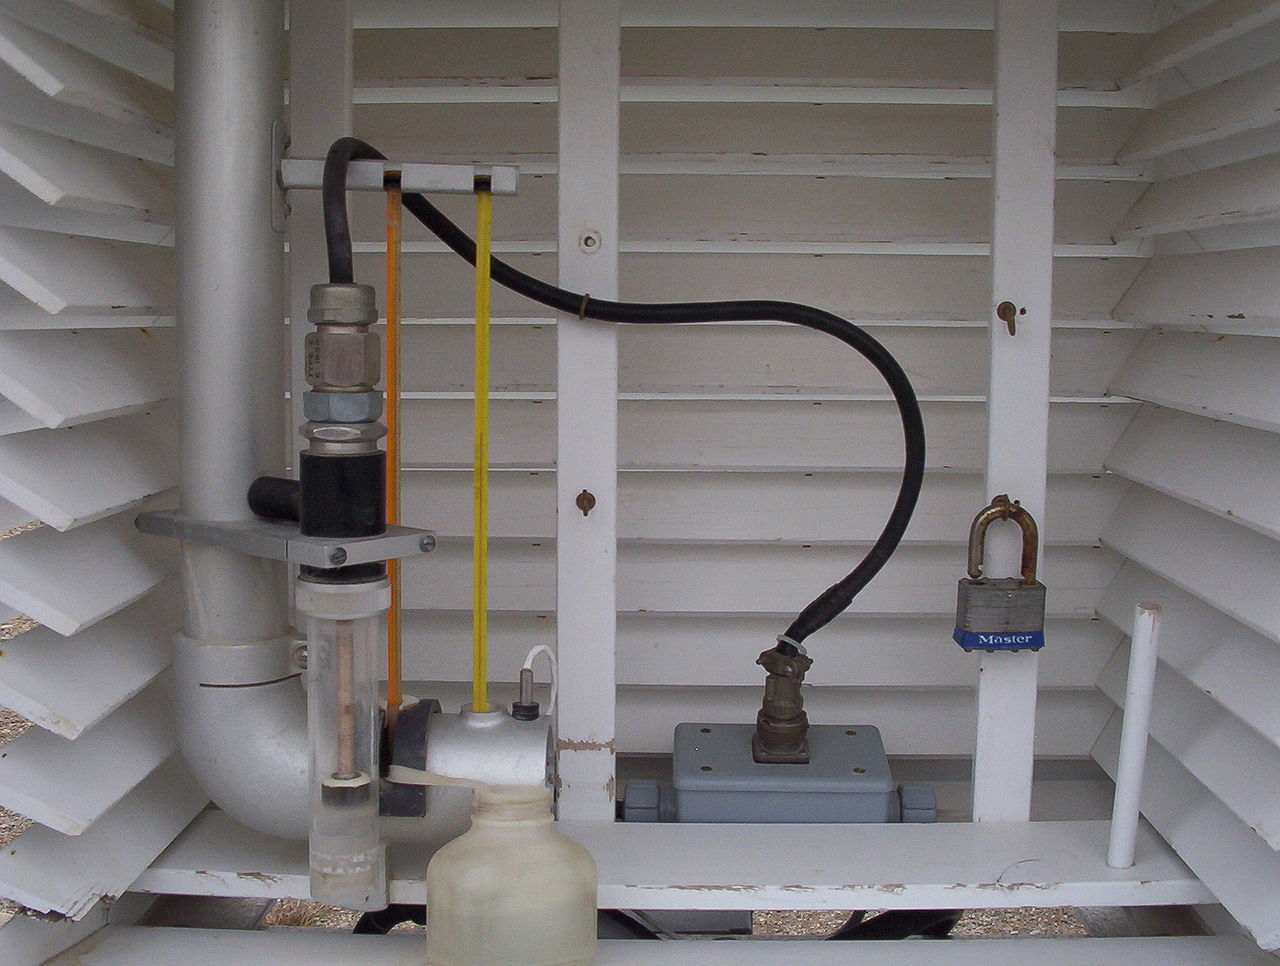
\includegraphics[height=7cm]{stevenson-screen-interior}
	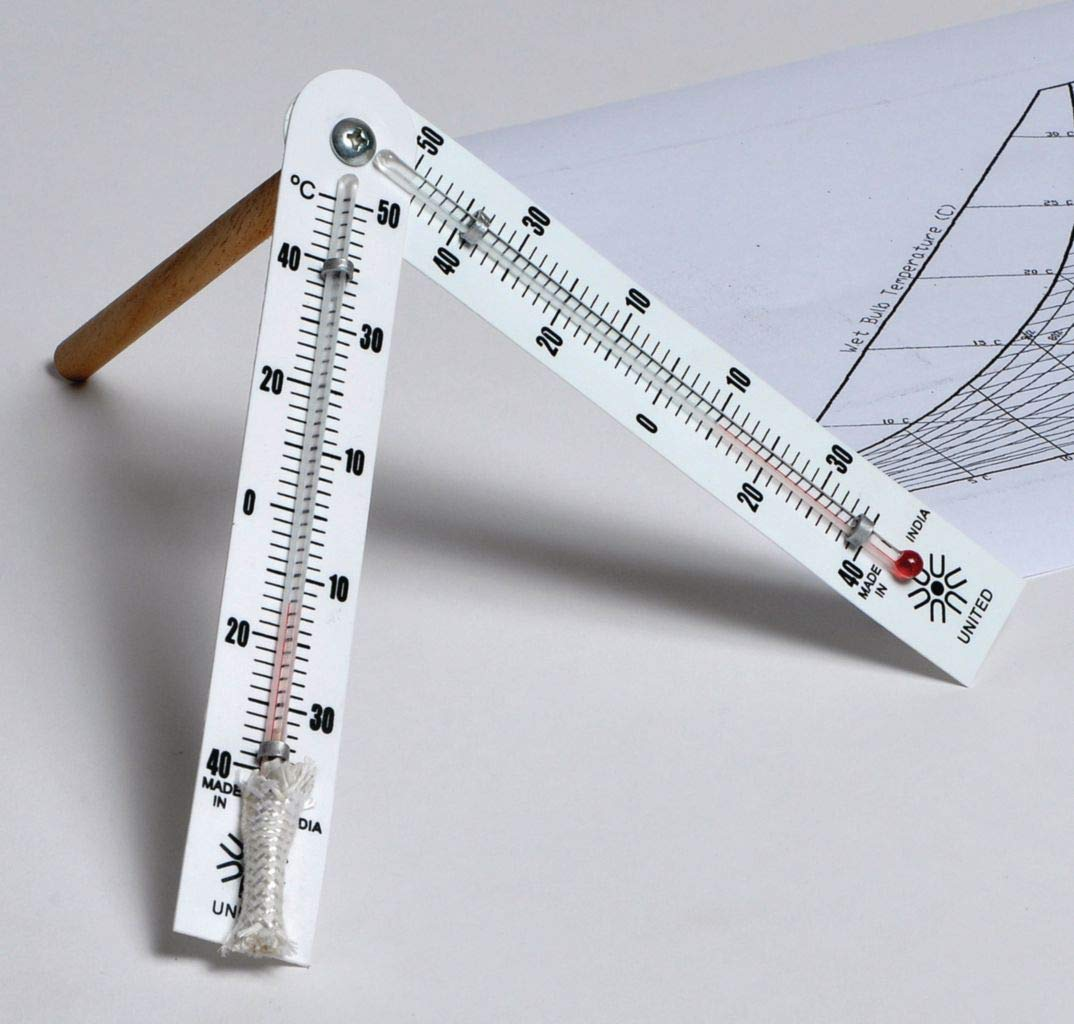
\includegraphics[height=7cm]{sling-psychrometer}
\end{center}

Voda na vyparenie vyžaduje energiu, tá pochádza z tepla. Takisto vieme, že voda sa vyparuje pomalšie, keď je okolitý vzduch viac vlhký.
Takže, keď zoberieme dva teplomery, na jeden z nich nakvapkáme vodu, počkáme kým daná voda sa vyparí a porovnáme hodnotu na tomto teplomeri s druhým (suchým) teplomerom, tak by sme mali vedieť všetko nato, aby sme určili (relatívnu) vlhkosť vzduchu.

Ja som si jeden takýto psychrometer zbastlil:\\
\begin{center}
	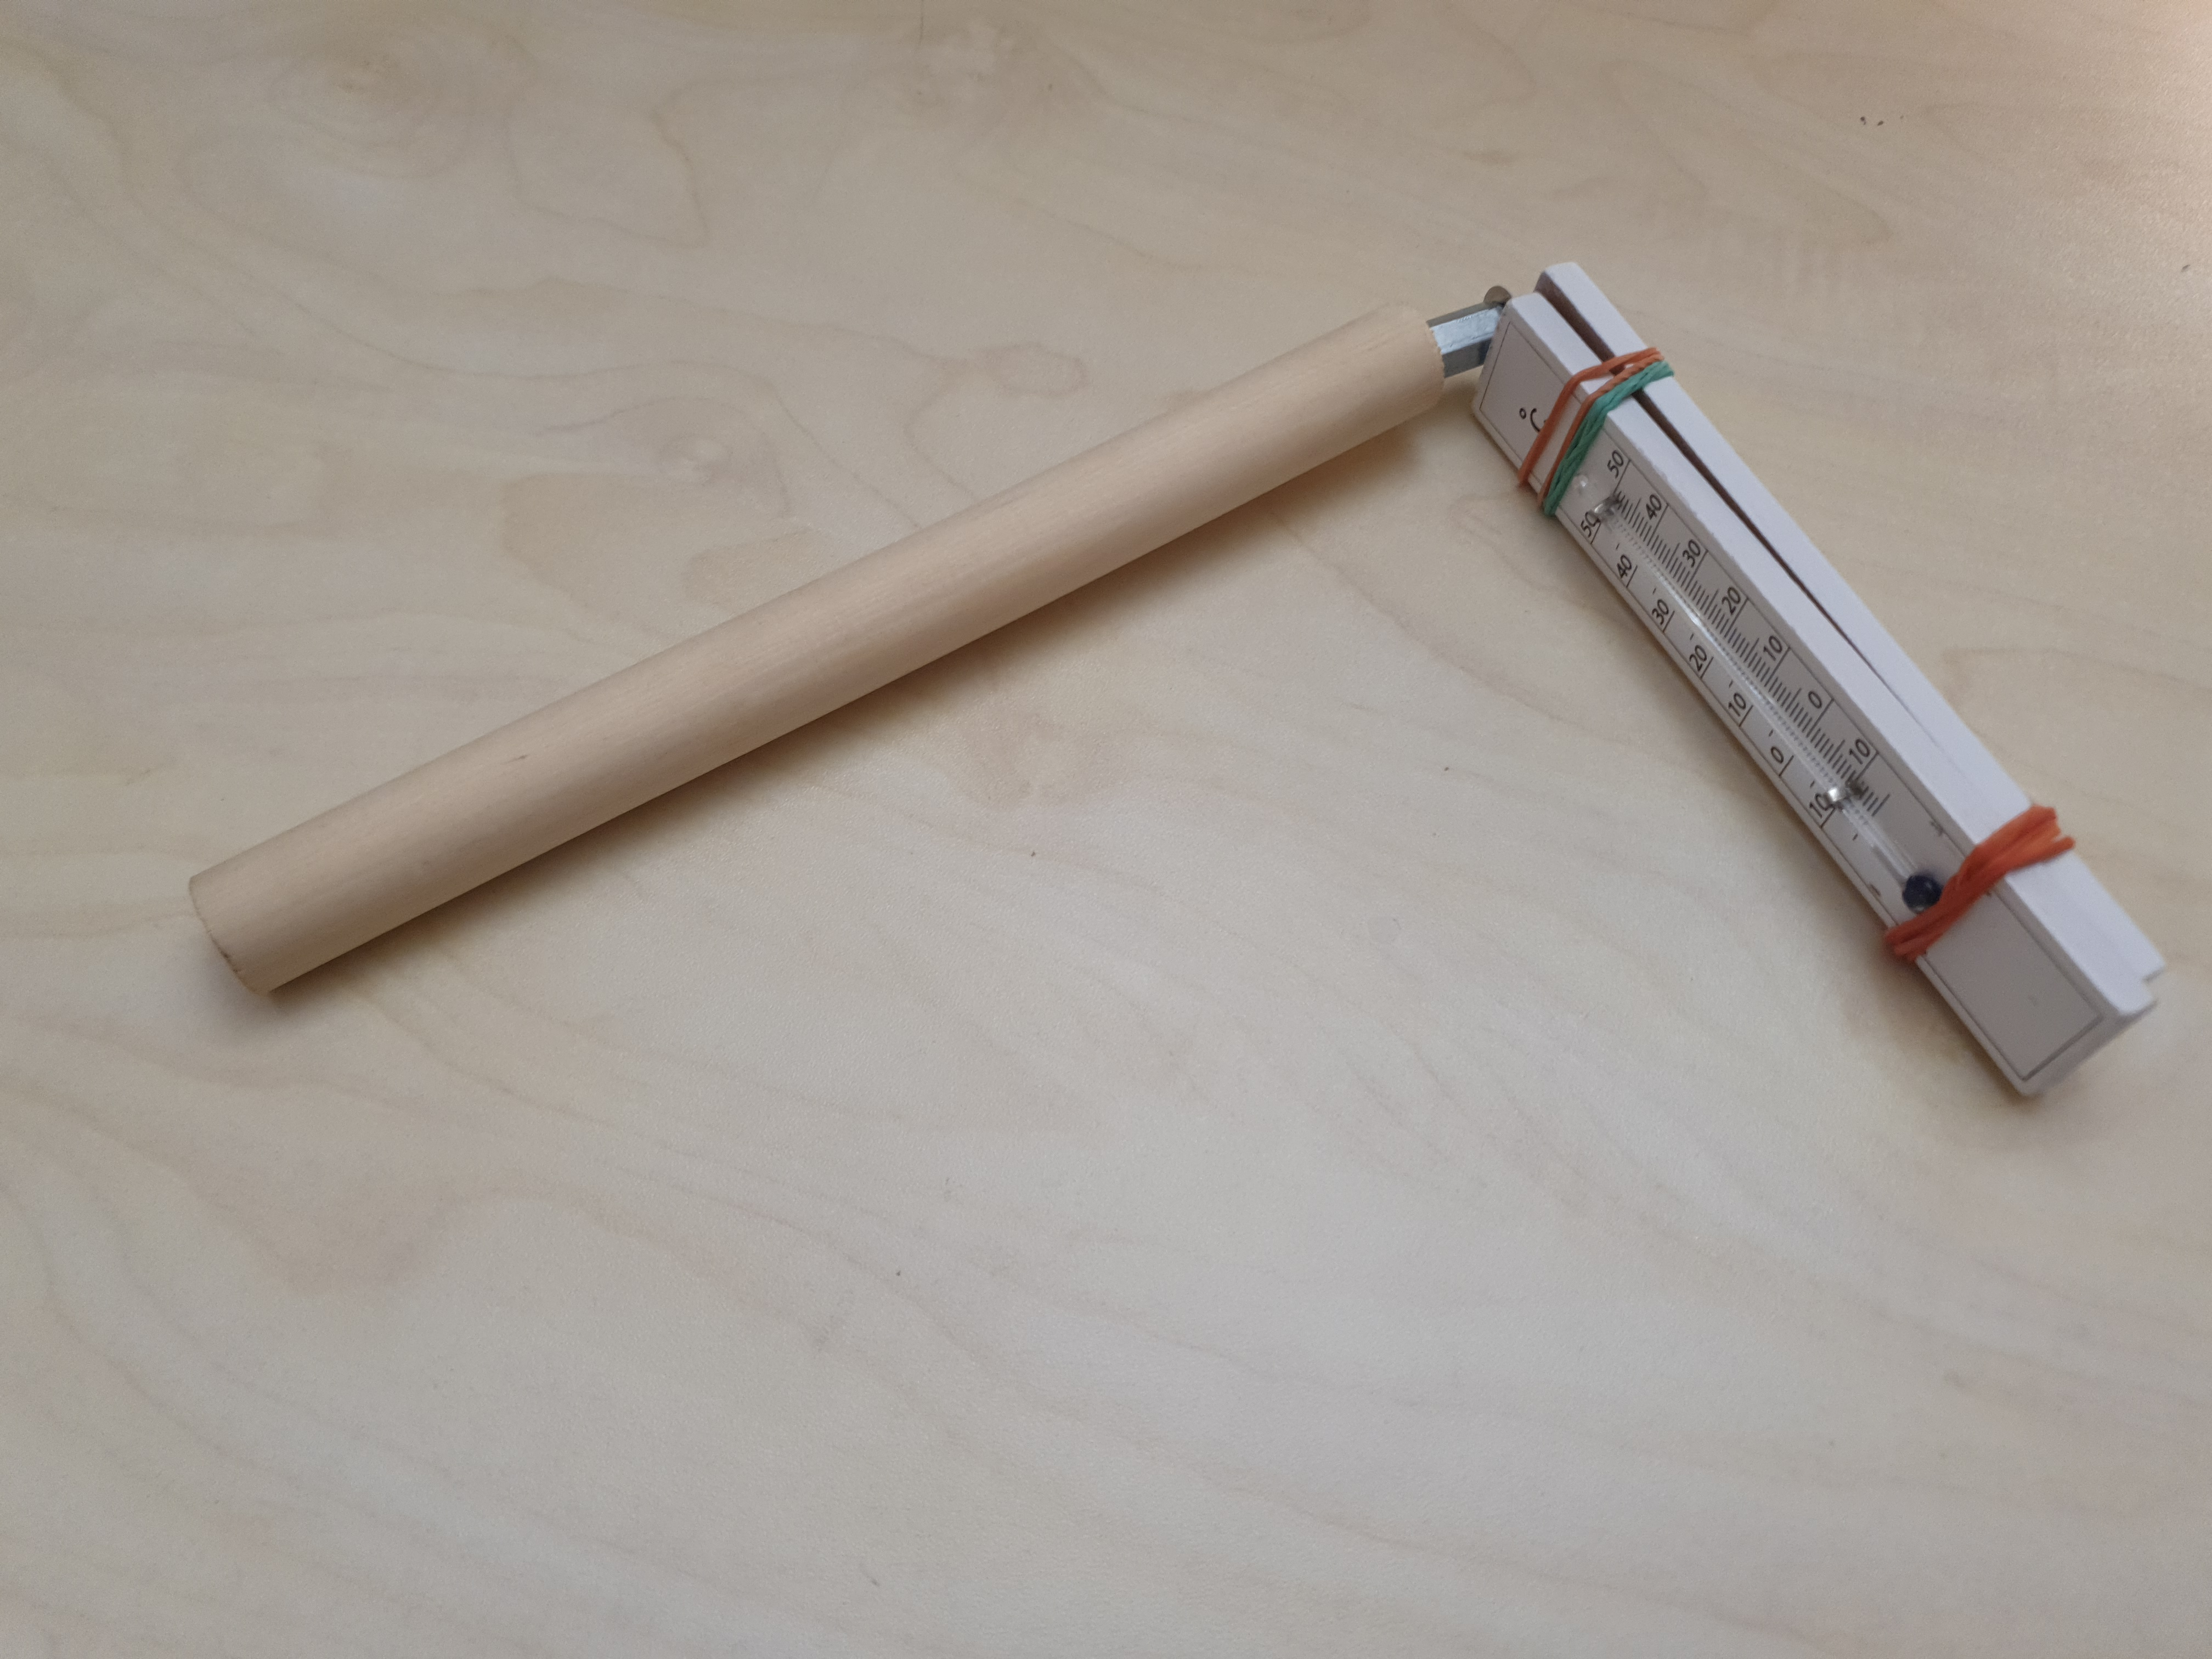
\includegraphics[height=4.5cm]{moj-sling-psychrometer-1}
	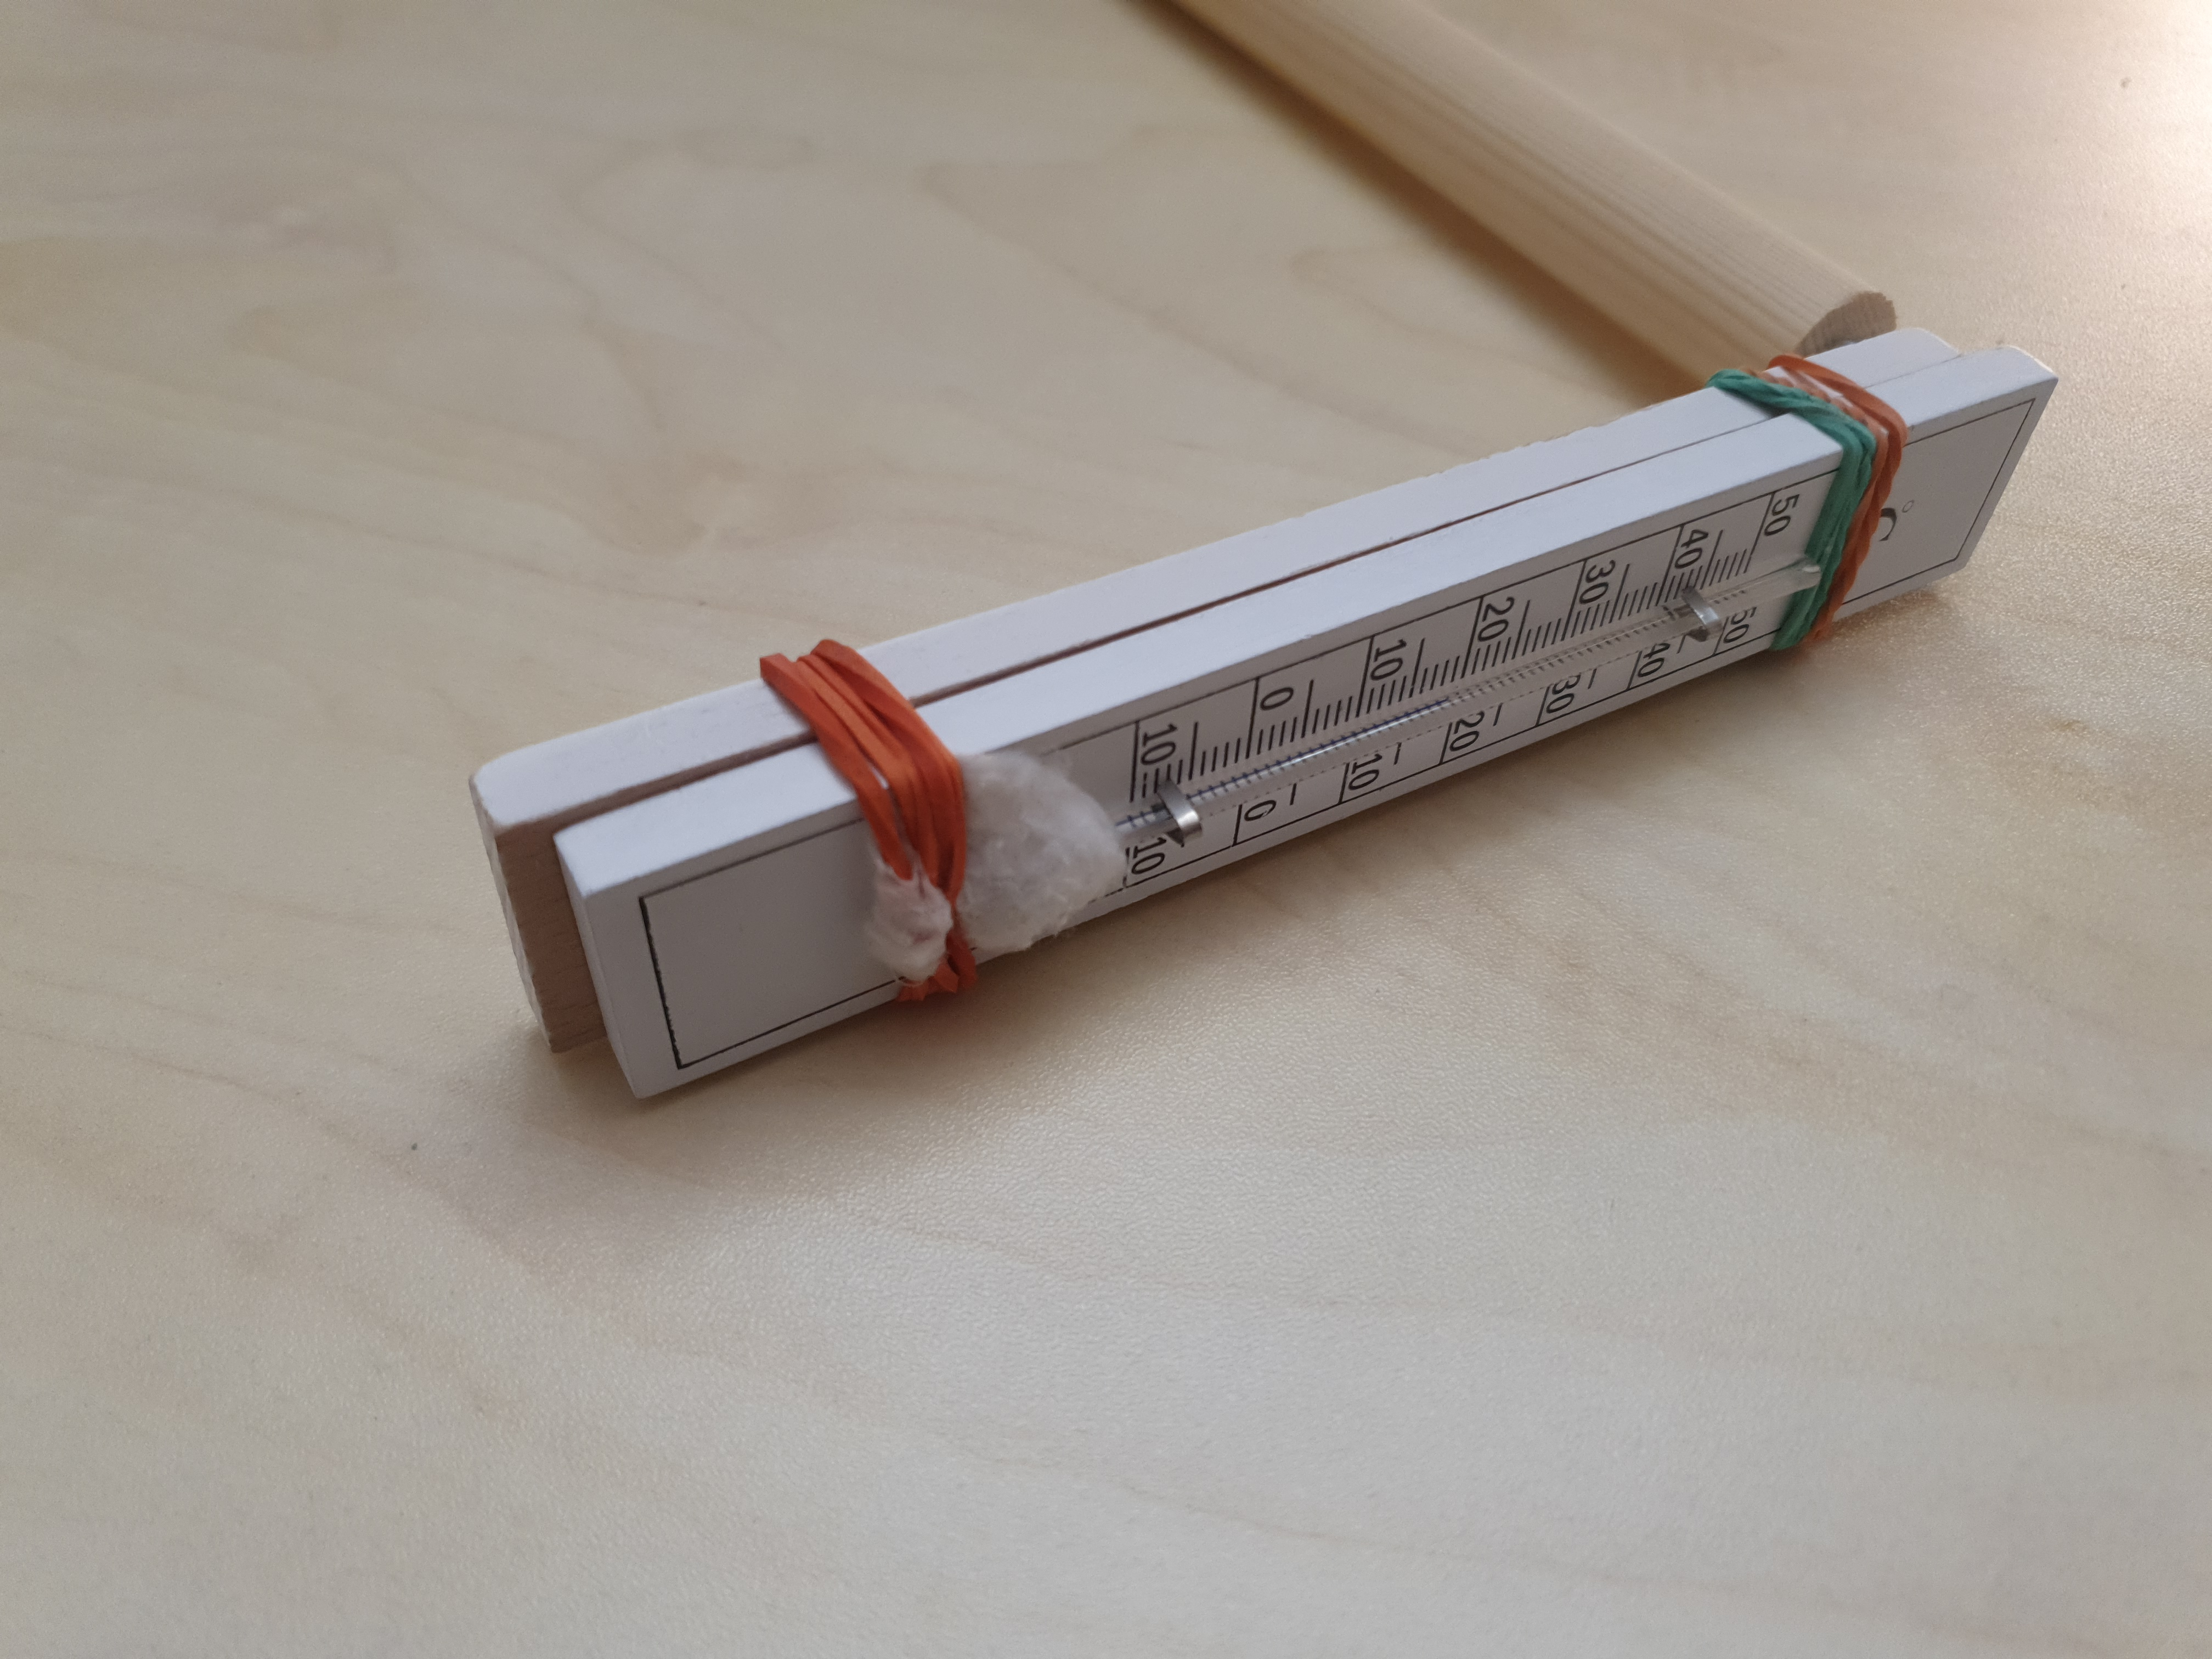
\includegraphics[height=4.5cm]{moj-sling-psychrometer-2}
	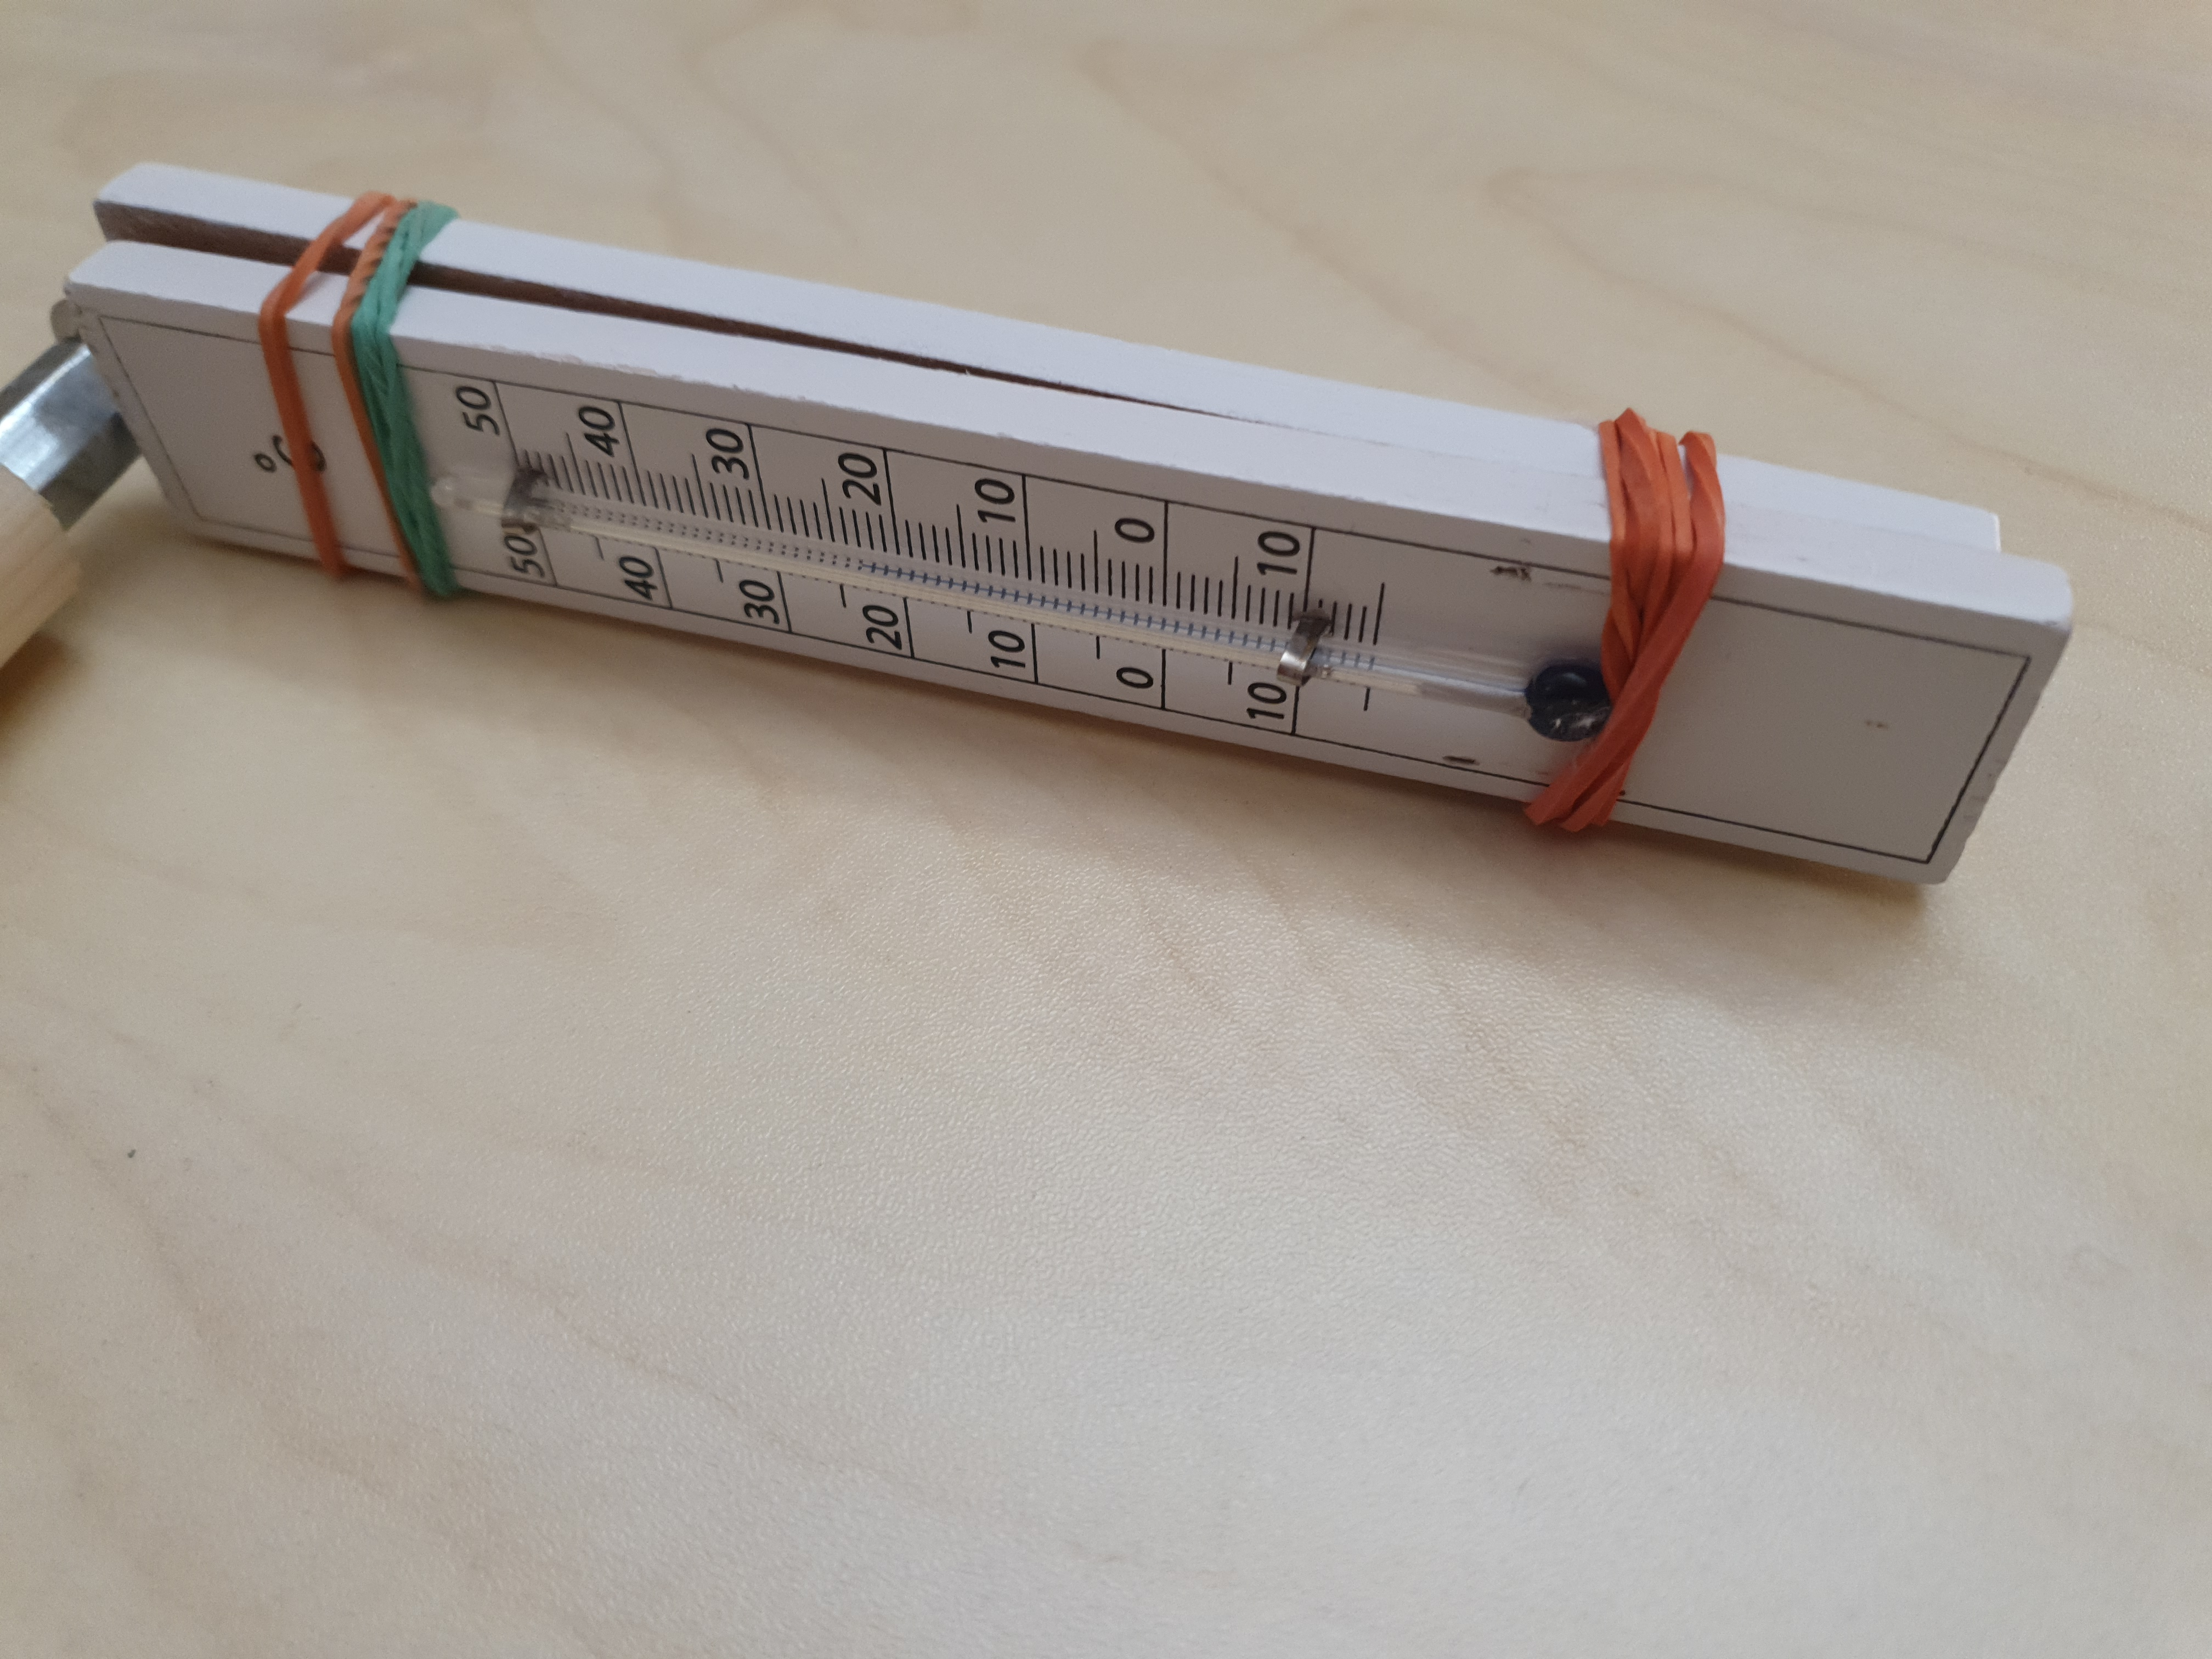
\includegraphics[height=4.5cm]{moj-sling-psychrometer-3}
\end{center}
Pri meraní treba vatu na jednej strane navlhčiť a potom "takú dobrú minútu" s teplomermi rýchlo točiť.
Točením sa vyparovanie vody urýchluje, bez toho aby to ovplyvnilo nameranú hodnotu.
Po meraní si treba teplotu obidvoch teplomerou zapísať.
Relatívna vlhkosť sa potom dá vyčítať z nasledovnej tabulky.
\begin{center}
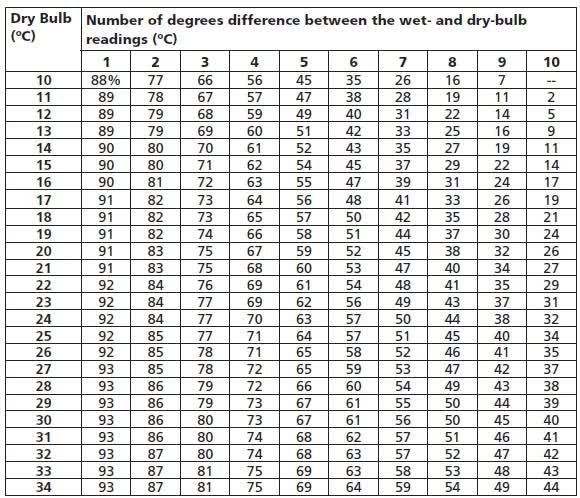
\includegraphics[width=0.9\textwidth]{relative-humidity-table}
\end{center}
Dry bulb je "suchý teplomer", wet bulb je "vlhký teplomer".
Moje hodnoty, namerané vonku, boli 9\textdegree C pre suchý teplomer a 7.5\textdegree C pre vlhký teplomer. Relatívna vlhkosť by mala byť podla tabulky medzi 80\% a 82\%. 
Relatívna vlhkosť v čase merania (2.11.2024 o 19:00) v Bratislave bola 83\% \cite{pocasie}.
Spomenul som pojem "relatívna vlhkosť", čo to je a aký je rozdiel medzi absolútnou a relatívnou vlhkosťou vysvetlím v nasledujúcej sekcií.
\section{Absolútna vs relatívna vlhkosť}
\textit{''Absolútna vlhkosť je hmotnosť vodných pár v objeme vlhkého vzduchu. Označuje sa $\rho_{p}$ a má jednotku $kg*m^3$.''} \cite{wiki-vlhkost}
Prvý vlhkomer, ktorý som v predošlej sekcií spomenul, by sa mohol použiť na meranie absolútnej vlhkosti. Keby sme dali kus uhlíka do $1m * 1m * 1m$ izolovanej krabice a počkali kým nenasiakne doňho všetka voda zo vzduchu vnútri tejto krabice, tak potom by pridaná hmotnosť z vody v uhlíku bola hodnota absolútnej vlhkosti vo vzduchu v tejto krabici pred meraním.\\
Teda absolútna vlhkosť vzduchu sa určuje vydelením hmotnosti vody vo vzduchu, objemom tohto vzduchu.\\

Relatívna vlhkosť bere do úvahy aj kapacitu vzduchu udržať viac pary.
\textit{''Relatívna vlhkosť je pomer množstva vlhkosti k maximálnemu možnému množstvu pri rovnakej teplote. Označuje sa $\phi$ a udáva sa v percentách.''} \cite{wiki-vlhkost}
Pri relatívnej vlhkosti 100\% je vzduch uplne saturovaný parou (vznikajú potom zrážky). Pri relatívnej vlhkosti 0\% neobsahuje vzduch žiadnu vodnú paru.
\\
Pri popisovaní počasia sa používa relatívna vlhkosť, lebo naše telo lepšie vníma množstvo vody, ktorá sa vyparuje z našeho tela ako množstvo pary vo vzduchu. \cite{quora}

\section{Záver}
Teraz už viete niečo o téme vlhkosti vzduchu a pri najblišiom pozeraní predovedi počasia v telke, môžte začať rozsiahlu debatu na túto tému.

\begin{thebibliography}{3}
	\bibitem{pocasie}{https://pocasie.sme.sk/krajina/slovensko/bratislava}
	\bibitem{wiki-vlhkost}{https://sk.wikipedia.org/wiki/Vlhkos\%C5\%A5\_vzduchu}
	\bibitem{quora}{https://www.quora.com/Why-is-relative-humidity-and-not-absolute-humidity-measured-in-weather-recording}
\end{thebibliography}

\end{document}
